\documentclass[12pt,journal,compsoc]{IEEEtran}
\usepackage{graphicx}
\usepackage{hyperref}
\ifCLASSOPTIONcompsoc

\else
 
\fi

\ifCLASSINFOpdf

\else

\fi

\newcommand\MYhyperrefoptions{bookmarks=true,bookmarksnumbered=true,
pdfpagemode={UseOutlines},plainpages=false,pdfpagelabels=true,
colorlinks=true,linkcolor={black},citecolor={black},pagecolor={black},
urlcolor={black},
pdftitle={Bare Demo of IEEEtran.cls for Computer Society Journals},%<!CHANGE!
pdfsubject={Typesetting},%<!CHANGE!
pdfauthor={Michael D. Shell},%<!CHANGE!
pdfkeywords={Computer Society, IEEEtran, journal, LaTeX, paper,
             template}}%<^!CHANGE!

\hyphenation{op-tical net-works semi-conduc-tor}


\begin{document}
\title{Risk perception in Cyber security environments using NLP}


\author{Gerard~Tio~Nogueras}

\IEEEcompsoctitleabstractindextext{%
\begin{abstract}
%\boldmath
This paper is a review of the natural language processing(NLP) techniques in risk perception and the cyber security risk assessment methods. This review attempts to unite these two fields to solve a scalability problem when it comes to the repeatability of the original experiment. The experiment consisting of a board game testing the risk-based mindset of the players and the social interactions that result during the game.
\end{abstract}

\begin{IEEEkeywords}
Natural Language Processing, nlp libraries, risk perception, risk assessment, ISO27001.
\end{IEEEkeywords}}

\maketitle

\IEEEdisplaynotcompsoctitleabstractindextext

\IEEEpeerreviewmaketitle

\section{Introduction and motivation}

\IEEEPARstart{W}{here} does this research come from?
"Stakeholders’ in security decisions play a fundamental role in determining security requirements, yet, little is currently understood about how different stakeholder groups within an organisation approach security and the drivers and tacit biases underpinning their decisions"\cite{DnD}. To have a better understanding of this subject, Dr. Sylvain \textsc{Frey} has created a board game that simulates these interactions. \\
The problem his team encountered when proposing their results to the main cyber security conferences is that their results were not accepted because of the low amount of games played resulting in not enough evidence.
Therefore this project is an attempt to circumvent the issue and support their results. The candidate approached in this review is NLP because it only needs a large amount of text which the scripts of the game provide.

\section{Overview of NLP}
\subsection{Concept of NLP}
NLP stands for natural language processing, it is a sub-field in artificial intelligence. It focuses on the analysis of natural language and the interactions between natural language and computers. It is an expanding research topic in any human related field.  NLP is achieved with the combinations of algorithms to solve the syntax(parsing, tagging, sentence breaking, ...), the semantics(lexical semantics, translations, language understanding, ...), the discourse(summarization, analysis of the connection between parts of the discourse, ...) or  the speech(speech recognition, speech segmentation, ...) depending on the problem faced.\cite{def}
\subsection{Reason to the NLP approach}
The average length of the games is two hours long and needs a trained game master, this makes the scaling of the number of games played very hard. NLP should enable a way to counter this problem. To transpose the study to NLP, some games were recorded and the scripts are available to be exploited by NLP algorithms. The goal is to use NLP to produce a report of the interactions by profiling the players and their risk-based decisions. The objective is to visualise the starting state of the players, their adaptations, their knowledge, the interactions with the "champion"(natural leader among the players), their risk assessment, how different backgrounds affect the decision-making process, as well as their progress along the game\cite{DnD}.
\subsection{Comparison of open source NLP libraries}
Here are some of the main open source libraries for NLP:
Standford Core NLP, Natural Language Toolkit(NLTK), Apache OpenNLP and Freeling. The comparison of these libraries will determine the most appropriate one for the project or the most appropriate according to the challenges faced during the project.
\subsubsection{Standford Core NLP}
\paragraph{Core: \\This library has the main tools necessary for an NLP project. It is built for Java but has wrappers for many other languages. It is based on annotators that are customizable for different usages thanks to a good amount of properties available\cite{Standford}}
\paragraph{Features: \\For the English language these are the main available features}
\begin{center}
\includegraphics[scale=0.35]{stdford.png} 
\end{center}
\subsubsection{NLTK}
\paragraph{Core:\\ NLTK is a python library based on a set of independent modules that take care of the main processing. To this modules are attached sub-modules for more specific tasks. The core of nltk is its ease of use by focusing on the students access to the toolkit along their course, its consistency, its capacity to extend, its documentation and its modularity (the independence of the modules allow the user no to worry about the whole toolkit when writing projects). One of the main downsides of the toolkit is that it is not optimised for efficiency\cite{nltk}} 
\paragraph{Features:\\ The main modules of the toolkit are the following: Accessing corpora, string processing, collocation discovery, speech tagging, classification, chunking, parsing, semantic interpretation, evaluation metrics, probability and estimation, applications and linguistic fieldwork.\\
%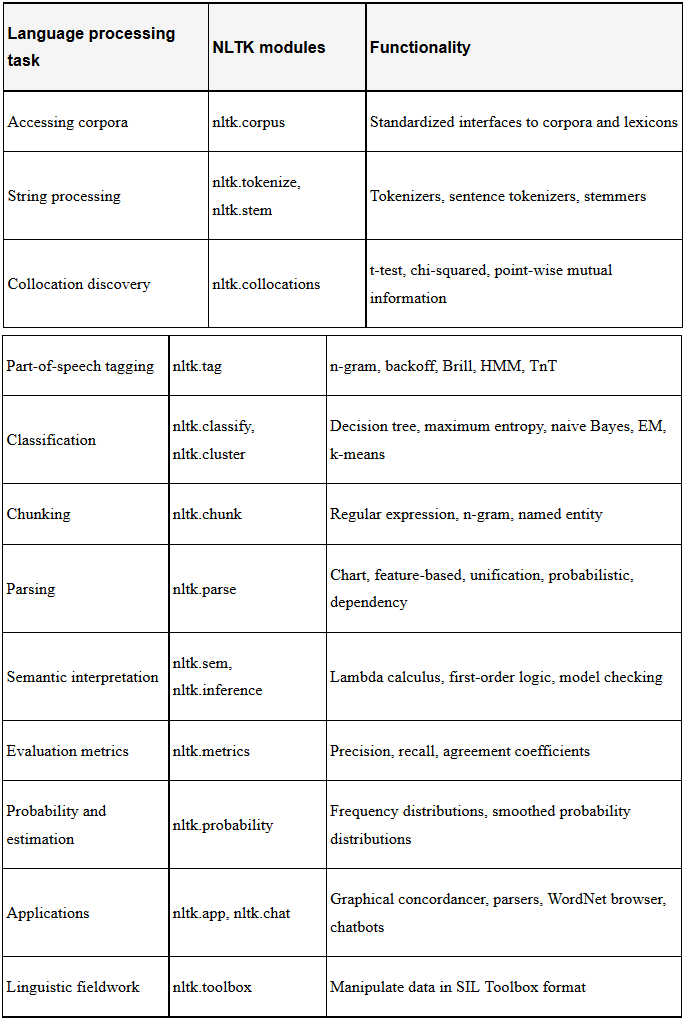
\includegraphics[scale=0.3]{nltk.png}{h}
\cite{nltk book}}
\subsubsection{Apache OpenNLP}
\paragraph{Core:\\OpenNLP is a Java library with the general tools needed to execute language processing and also the tools to extend projects to more advanced processing needs.\cite{Opennlp}}
\paragraph{Features:\\Sentence detector, tokenizer, Name finder, document categorizer, part-of-speech tagger, lemmatizer, chunker, parser, coreference resolution, corpora. }

\subsubsection{Freeling}
\paragraph{Core: \\
Freeling is a library divided into 2 types of objects: linguistic and processing. The linguistic data classes are used to interpret the sentences and their structure(words, sentences, tags, ...). The processing classes allow the transformation of the linguistics objects(token, splitting, tagging, ...). The library is written in C++ but is portable to other languages and facilitates its customization.\cite{Freeling}}
\paragraph{Features:\\
Tokenization, Morphological analysis, Multiword recognition, proper noun detection, Date-time expression recognition, Currency expression recognition, Numerical expression recognition, Part-of-Speech tagging.}


\subsection{Libraries summary}
Every library has its advantages and their use will depend on the specific needs encountered during the project. The main choice will probably be NLTK because of the ease of use, a very good documentation and a large number of features available as well as the ease to customize the modules if needed.
%\\\\
%\begin{tabular}{ |c|c|c|c| } 
% \hline
%  & Standford & NLTK & OpenNLP  \\
% \hline 
% \hline 
% feat1 & X & X & X  \\
% \hline 
% feat2 & X & X & X  \\
% \hline 
% feat1 & X & X & X  \\
% \hline 
% feat2 & X & X & X  \\
% \hline 
% feat1 & X & X & X  \\
% \hline 
% feat2 & X & X & X  \\
% \hline
%\end{tabular}
%\\\\\\
%\begin{tabular}{ |c|c| } 
% \hline
%  &  FreeLing  \\
% \hline 
% \hline 
% feat1 & X   \\
% \hline 
% feat1 & X   \\
% \hline 
% feat1 & X   \\
% \hline 
% feat1 & X  \\
% \hline 
% feat1 & X  \\
% \hline 
% feat1 & X   \\
% \hline
%\end{tabular}
\section{Risk management overview}
Risk management is based on the standard ISO27001. \cite{iso}
\subsection{Main standard in risk }
The risk events in the game are already discussed in \cite{DnD} using the recommendation of the ISO27001. Here the standard will be used to track the player's process during budget decisions. 
There are two aspects of the standard that will be utilised in the project. The risk matrix and the IT security management cycle.
The matrix allows to easily categorise threats and decide if action is needed depending on its likelihood and its impact on the company.
\\\\
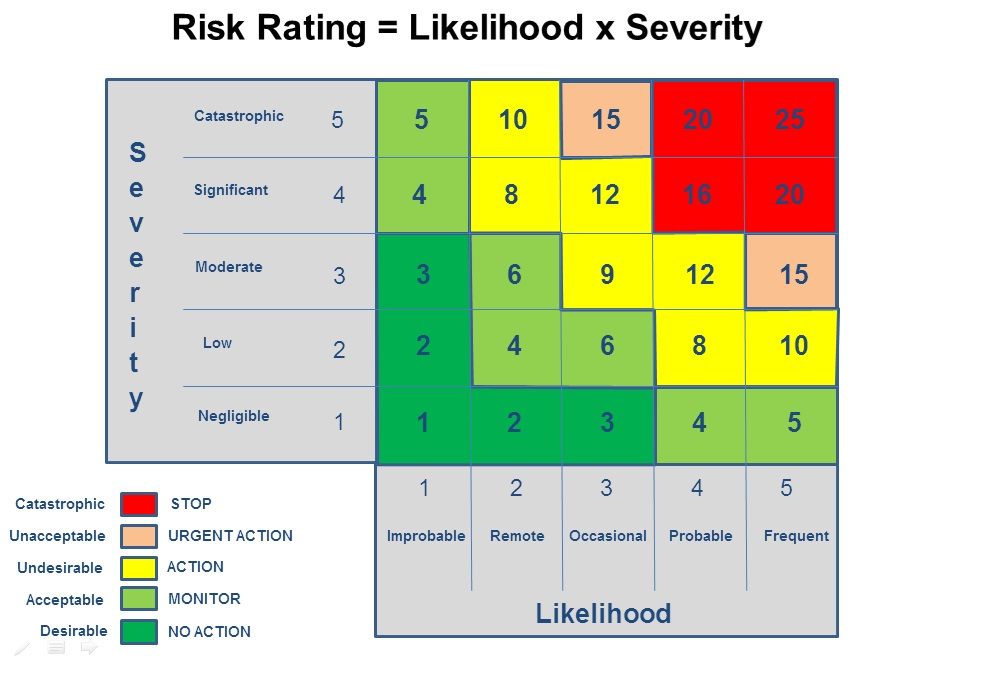
\includegraphics[scale=0.35]{risk-matrix.png}
The second tool is the IT security management cycle, which proposes steps to assure every aspect of security is covered during a risk assessment. The players will not be expected to follow the steps but will be compared to a simplification of the cycle.\cite{cycle}
%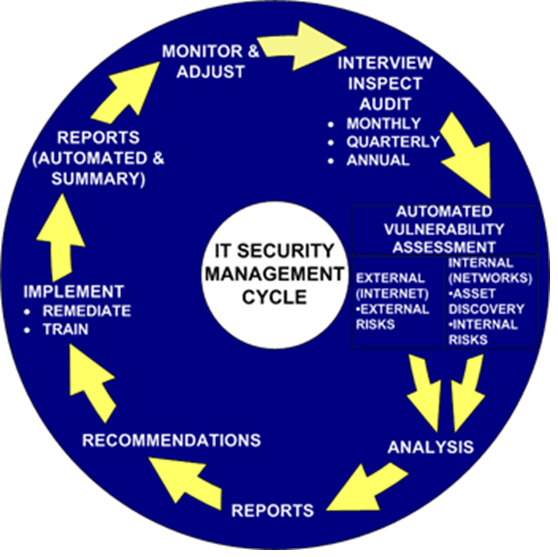
\includegraphics[scale=0.3]{cycle.png}
\section{Conclusion}
The next steps will be to test out the NLP algorithms and study how to use the extracted data to create reports on the games played and the player's perceptions, decisions and discussions. Another aspect that we hope to achieve is to create a starting ground for future research on risk-based profiling for cyber security decisions. Because right now there is a lot of research done on medical risk but not for cyber security risk perception.
\\\\
The final goal of this research is to support the results found previously and additionally to be able to create reports with constructive criticism of the flaws of the player's methodology and the approaches taken during the game to enhance the risk-based decisions of the different entities of the company.

\begin{thebibliography}{1}

\bibitem {DnD} Sylvain Frey, Awais Rashid, Pauline Anthonysamy, Maria Pinto-Albuquerque, and Syed Asad Naqvi. 2016.  The Good, the Bad and the Ugly: A Study of Security Decisions in a Cyber-Physical Systems Game.

\bibitem {def} Web.stanford.edu. (2017). CS224n: Natural Language Processing with Deep Learning. Available at: \url{http://web.stanford.edu/class/cs224n/syllabus.html} (Accessed 2 May 2017). 

\bibitem {iso} Iso.org. (2013). ISO/IEC 27001:2013. Available at: \url{https://www.iso.org/obp/ui/\#iso:std:iso-iec:27001:ed-2:v1:en} (Accessed 2 May 2017).

\bibitem {matrix} Faa.gov. (2016). Develop Preliminary Vulnerability and Risk Assessment (e). Available at: \url{https://www.faa.gov/about/office_org/headquarters_offices/ato/service_units/operations/isse/items/e-Dev-Prem-Vul-Risk-assessment.cfm?print=go\&sa=U&ei=bSV-VLDRL6TMygOWj4CoCQ\&ved=0CCsQ9QEwCw\&usg=AFQjCNFB1GZabJ5pruv5JfvOvYP68gUi3Q} (Accessed 2 May 2017).

\bibitem {nltk book} Steven Bird, Ewan Klein, Edward Loper. Natural Language Processing with Python : Analyzing Text with the Natural Language Toolkit, 17-18, 12 June 2009. O'Reilly Media, Inc.

\bibitem {nltk} Loper Edward and Bird Steven. NLTK: The Natural Language Toolkit. Proceedings of the ACL-02 Workshop on Effective Tools and Methodologies for Teaching Natural Language Processing and Computational Linguistics - Volume 1,2002,63-70,Association for Computational Linguistics. Available at: \url{http://dl.acm.org/citation.cfm?id=1118117} (Accessed 2 May 2017).

\bibitem {Standford} Manning, Christopher D., Mihai Surdeanu, John Bauer, Jenny Finkel, Steven J. Bethard, and David McClosky. 2014. The Stanford CoreNLP Natural Language Processing Toolkit In Proceedings of the 52nd Annual Meeting of the Association for Computational Linguistics: System Demonstrations, pp. 55-60. Available at: \url{https://nlp.stanford.edu/pubs/StanfordCoreNlp2014.pdf} (Accessed 2 May 2017).

\bibitem {Opennlp} Apache OpenNLP Developer Documentation Written and maintained by the Apache OpenNLP Development Community Version 1.7.2. Available at: \url{https://opennlp.apache.org/documentation/1.7.2/manual/opennlp.html}

\bibitem {Freeling} Lluis Padro and Evgeny Stanilovsky. FreeLing 3.0: Towards Wider Multilinguality. Proceedings of the Language Resources and Evaluation Conference (LREC 2012) ELRA. Istanbul, Turkey. May, 2012. Available at: \url{http://nlp.lsi.upc.edu/publications/papers/padro12.pdf} (Accessed 2 May 2017)

\bibitem {cycle} \url{http://www.torycredit.com/supplier-vendor-assesment-report/}
\end{thebibliography}


\end{document}


